%%%%%%%%%%%%%%%%%%%%%%%%%%%%%%%%%%%%%%%%%%%%%%%%%%%%%%%%%%%%%%%%%%%%%%%%%%%%%%%
% intro.tex: Introduction to the thesis
%%%%%%%%%%%%%%%%%%%%%%%%%%%%%%%%%%%%%%%%%%%%%%%%%%%%%%%%%%%%%%%%%%%%%%%%%%%%%%%%
\chapter{Introduction}
\label{intro_chapter}

\begin{chapquote}{Richard Feynman}
``Science is what we have learned about how to keep from fooling ourselves.''
\end{chapquote}
%%%%%%%%%%%%%%%%%%%%%%%%%%%%%%%%%%%%%%%%%%%%%%%%%%%%%%%%%%%%%%%%%%%%%%%%%%%%%%%%
Particle physics is the study of the particles that make up the universe, as well as the forces that affect them. The most widely accepted model is known as the Standard Model(SM), and has been shown to accurately explain and predict many processes. However, despite this, the Standard Model is limited. For instance, it does not account for dark matter, dark energy or even gravity. Even some terms that are in Standard Model are not necessarily predictive, such as the mass and charge of some particles since those terms are related to free parameters. Another difficulty with the standard model is even if all the terms are known, sometimes the calculations are difficult if not impossible such as many interactions involving the strong force. For this reason many models do not use the Standard Model for predicting certain effects of the strong force. 

An important concept when discussing the Standard Model is that although it doesn't predict the mass of particles directly, it does predict the relationship between some of the masses. For example by measuring the mass of the top quark and the Higgs Boson it is possible to predict the mass of the W. Figure \ref{fig:gfitterResults} shows a relationship between the theoretical mass of the W and the top quark for 4 different masses of the Higgs boson. With the mass of the Higgs measured as 125 GeV it is possible to predict the mass of the W given the measured mass of the top quark. As can be seen the measured mass of the W is over one sigma away from the predicted mass. While tantalizing, the significance of the disagreement is insufficient to currently demand the presence of new physics to explain it. The clearest way to resolve the disagreement would be to lower the error on the W boson's measured mass. \par
\begin{figure}[!htbp]
    \centering
    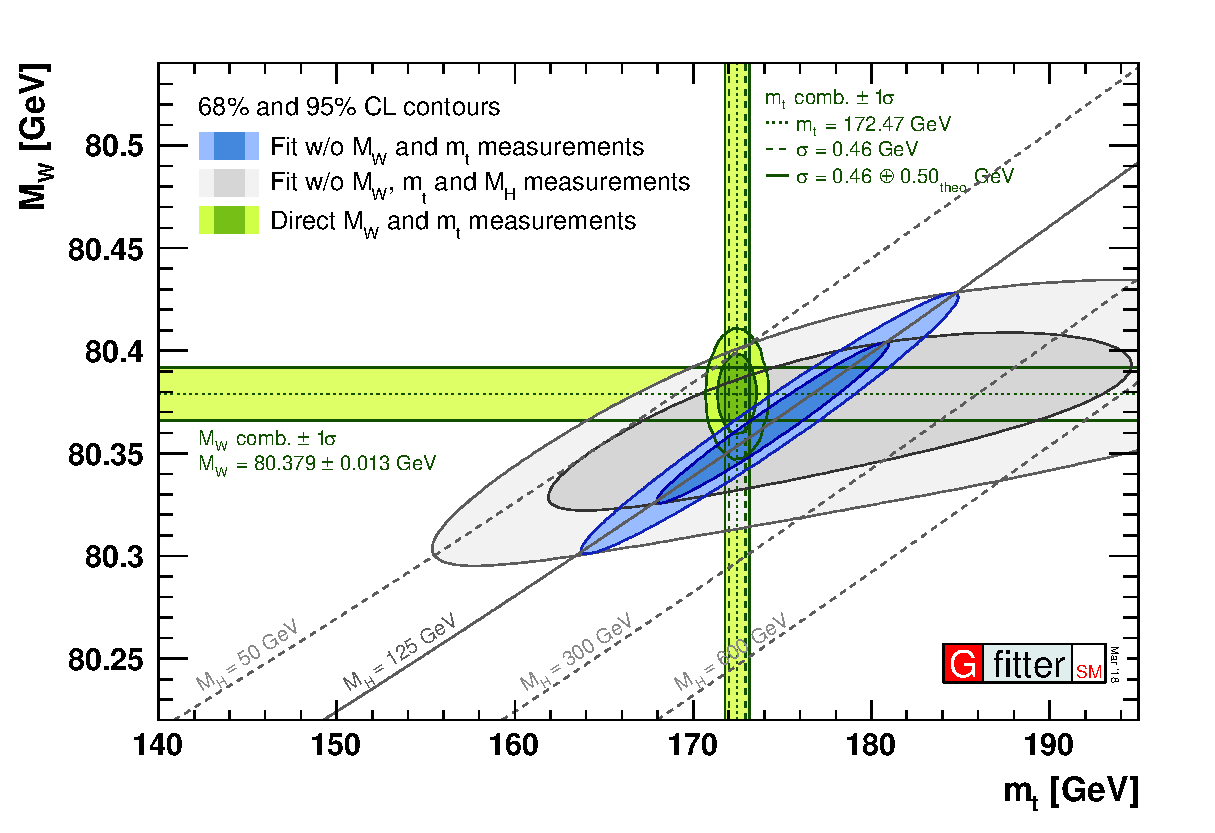
\includegraphics[width=\textwidth]{figures/TheoryFigures/2018_03_20_Scan2D_MWvsmt_logo.eps}
    \caption[
        W mass gFitter results
    ]{
     Current measured mass of the W boson and top quark using gfitter, compared to the theoretical values. With the current measured mass of the Higgs boson, 125 GeV, the theory does not match the experimentally measured masses of the W boson and the top quark. 
    }
    \label{fig:gfitterResults}
\end{figure} Measuring the mass of the W is difficult to do with a hadron collider however, since it requires accurate predictions of the effect of low energy strong interactions.  This thesis attempts to test the effects of modifying the ``hadronizer" which simulates the effects of low energy strong interactions. These effects are probed by measuring the leptons that result from a \Z decay. Both the \Z and its decay products lack any direct interaction with the strong force.  Therefore once the Z is produced, the strong force will have only a trivial effect on the measured value. Thus, by measuring the momentum of the leptons we can calculate the transverse momentum of the \Z(\bosonpt) and can then infer information about the transverse momentum of the particles that produced it. In place of measuring the \bosonpt of the Z directly the novel variable \phistar is used\cite{PhiStarSource}. This variable, while being highly correlated with \bosonpt, has a much smaller percentage uncertainty, allowing for more accurate tests of the transverse momentum  of the parent particles of the \Z.  

The data used was collected using the Compact Muon Solenoid detector(CMS) at the Large Hadron Collider(LHC) in 2012. The data used  contains $\SI{19.7}{fb}^{-1}$ of integrated luminosity at a center of mass energy of 8 TeV. 

The final measured result compares normalized \phistar differential cross-sections that was collected at the the CMS to different simulation softwares. One of the simulation softwares was used multiple times with different settings in an attempt to match the data more effectively.




%%%%%%%%%%%%%%%%%%%%%%%%%%%%%%%%%%%%%%%%%%%%%%%%%%%%%%%%%%%%%%%%%%%%%%%%%%%%%%%%
